
	\documentclass{article}
	\usepackage{amsmath,amssymb}
	\usepackage[inline]{enumitem}
	\usepackage{blindtext}
	\usepackage{booktabs}
	\usepackage{graphicx}
	\usepackage{xcolor}
	\usepackage[vmargin = 1.5in, top = 1in, bottom = 1.2in, letterpaper]{geometry}
	\usepackage{listings}
	\usepackage{courier}
	\usepackage{multicol}
	\usepackage{multirow}
	\usepackage{bm}
	\lstset{
	basicstyle = \small\tt,
	keywordstyle = \tt\color{blue},
	commentstyle = \it\color[cmyk]{1,0,1,0},
	stringstyle = \tt\color[RGB]{128,0,0},
	%frame = single,
	backgroundcolor = \color[RGB]{245,245,244},
	breaklines,
	extendedchars = false,
	xleftmargin = 2em,
	xrightmargin = 2em,
	aboveskip = 1em,
	tabsize = 4,
	showspaces = false
	}
	\begin{document}
	
	% \newfontfamily\courier{Courier New}

	
	\title{STAT 520 Homework 2}
	\author{Yifan Zhu}
	\maketitle
	
	\begin{enumerate}[leftmargin = 0 em, label = \arabic*., font = \bfseries]
	\item 
	$Y_{ij}$ are independent, and $Y_{11}, Y_{12}, \ldots , Y_{1n_{1}} \overset{i.i.d}{\sim} Gamma(\alpha_1, \beta_1),\, Y_{21}, Y_{22}, \ldots , Y_{2n_{2}} \overset{i.i.d}{\sim} Gamma(\alpha_2, \beta_2)$.

	We use $\alpha$ and $\beta$ to note the parameter of Gamma distribution for one group and $n$ be the size of that group. Then the log likelihood is 
	\[\ell (\alpha , \beta ) = n(\alpha \log \beta) - \log \Gamma(\alpha) + (\alpha - 1)\sum_{i=1}^n \log y_i - \beta \sum_{i=1}^n y_i\]


	\item 
    By the property of mle, we can obtain the standard error for $\hat{\alpha}$ and $\hat{\beta}$ in this way.

	By taking second derivative, we have
	\begin{align*}
	&\frac{\partial^2 \ell}{\partial \alpha^2} = -n \frac{\Gamma''(\alpha) \Gamma'(\alpha) - {\Gamma'(\alpha)}^2}{(\Gamma'(\alpha))^2}\\
	&\frac{\partial^2 \ell}{\partial \beta^2} = -\frac{n \alpha}{\beta^2}\\
    &\frac{\partial \ell}{\partial \alpha \partial \beta} = \frac{n}{\beta}
	\end{align*}

	Then we can get Fisher Information
	\[I_n = - \mathbb{E}_{\alpha, \beta}(Hessian(\ell))\]
	and 
	\[I_n^{-1} = \begin{bmatrix}
		\sigma_\alpha^2 & \sigma_{\alpha, \beta}\\
		\sigma_{\alpha, \beta} & \sigma_\beta^2
	\end{bmatrix}\]
	
	Then we can get the 95\% confidence interval for $\alpha$ and $\beta$ from $\hat{\alpha} \pm 1.96 \hat{\sigma}_\alpha$ and $\hat{\beta} \pm 1.96 \hat{\alpha}_\beta$. The results are listed in the table.
\begin{center}
	\begin{tabular}{ccccc}
	\toprule
	         & $\hat{\alpha}$ & $\hat{\beta}$ & CI for $\hat{\alpha}$ & CI for $\hat{\beta}$\\ 
	         \midrule
	 Group 1 &  4.56&  2.41&  (2.12, 7.01)& (1.04, 3.78)   \\
	 Group 2 &  1.04&  0.54&  (0.53, 1.55)& (0.20, 0.88)  \\
	 Combined & 1.65&  0.87&  (1.06, 2.25)& (0.50, 1.23)\\
	 \bottomrule
	\end{tabular}
	\end{center}

	\item Let $\ell_1$ and $\ell_2$ be log likelihood for group 1 and group 2. Then the log likelihood for the full model is
	\[\ell_{full} = \ell_1 (\hat{\alpha}_1, \hat{\beta}_1) + \ell_2 (\hat{\alpha}_2, \hat{\beta}_2) \]

	The log likelihood for redued model $\ell_{reduced}$ is that for the combined data. Thus we can get the deviance $G^2$ 
	\[G^2 = -2(\ell_{reduced} - \ell_{full}) = 14.33\]

	The difference in dimension of parameter is 2, thus $G^2 \overset{.}{\sim} \chi^2_{2}$.

	Meanwhile, $\chi_{1, 0.9}^2 = 2.7$, which is less than 14.33. Hence we reject the reduced model.


	\item 
	Graph as shown below.
	\begin{center}
		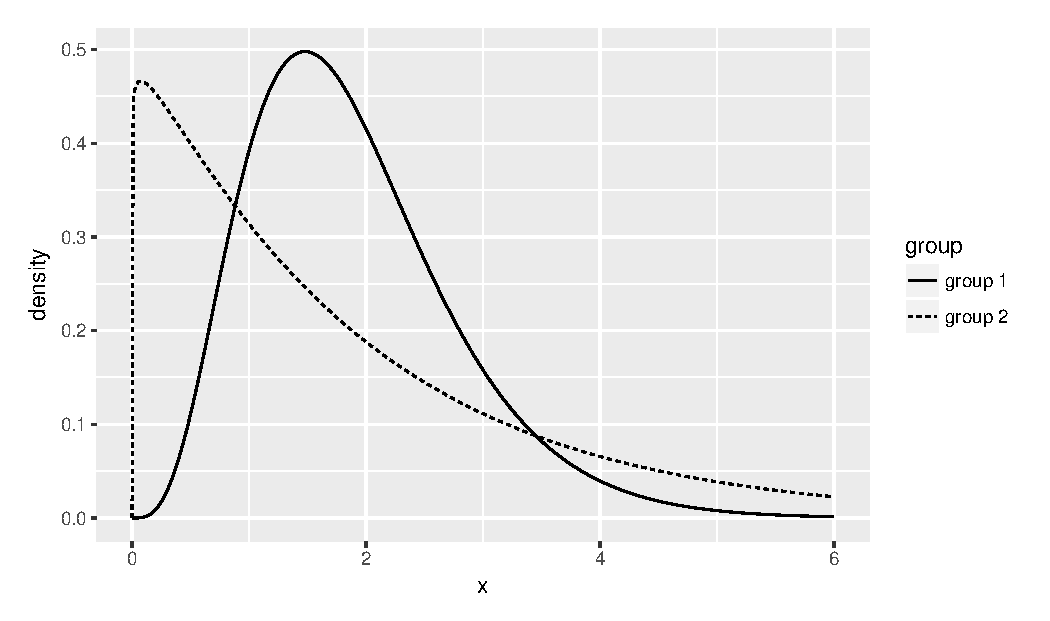
\includegraphics[width = .8\textwidth]{Rplot.eps}
	\end{center}


	\item 
	Let $\mu_i$ be the expected value for group $i$, then $\mu_i = \frac{\alpha_i}{\beta_i} = g(\alpha_i, \beta_i)$. Here $g$ is a continuous function. Then $\widehat{(\mu_1 - \mu_2)} = \hat{\mu}_1 - \hat{\mu}_2 = \frac{\hat{\alpha}_1}{\hat{\beta}_1} - \frac{\hat{\alpha}_2}{\hat{\beta}_2} $.

    Then we need $\hat{Var}(\hat{\mu}_1 - \hat{\mu}_2)$. Because of independece, $Var(\hat{\mu}_1 - \hat{\mu}_2) = Var(\hat{\mu}_1) + Var(\hat{\mu}_2)$. For any group, let $\mu$ be its mean, $\mu = \alpha / \beta = g(\alpha, \beta)$. Let 
    \[D = \begin{bmatrix}
    	\frac{\partial g}{\partial \alpha}\\
    	\frac{\partial g}{\partial \beta}
    \end{bmatrix} = 
    \begin{bmatrix}
    	\frac{1}{\beta}\\
    	-\frac{\alpha}{\beta^2}
    \end{bmatrix}\]

    Then by Delta Method, $Var(\hat{\mu}) = D^T I_n^{-1} D$.  By pluging in $\alpha_i, \beta_i$, we have $\hat{Var}(\hat{\mu}_1) = 0.0314, \hat{Var}(\hat{\mu}_2) = 0.1426$. Thus from $(\hat{\mu}_1 - \hat{\mu}_2) \pm 1.96 (\hat{Var}(\hat{\mu})_2 + \hat{Var}(\hat{\mu}_2))$, we know
    \[CI = (-0.854, 0.781)\]


    \item 
    Using the pooled sample variance by assuming equal variance of the two groups
    \[s^2_p = \frac{(n_1 - 1)s^2_1 + (n_2 - 1)s_2^2}{n_1 + n_2 - 2}\]
    Then 
    \[t = \frac{\bar{y}_1 - \bar{y}_2}{\sqrt{s_p^2/(n_1 + n_2)}} = -0.1782\]

    The t statistic here has a degree of freedom of 48, and p-value is 0.5704. We fail to reject the null hypothesis that $\mu_1 = \mu_2$. Thus it disagree with the results in 3, but since the confidence interval in 5 contains 0, thus it agrees with the result in 5. 


    \item 
    In this problem, we want to test if these two groups follow the same Gamma distribution. But in 5 and 6, the test is only for the difference in mean of these two groups. It restricts the cause of difference to be the difference in means, which I don't think is reasonable. In 3 we do not have such restriction. It tests if these two Gamma distribution is actually one Gamma distribution. This may also be the reason why 3 do not gave the same conclusion like 5 and 6. Hence I think the result from 3 is better for this problem and conclude that there is evidence taht these two Gamma distributions are different.


 	\end{enumerate}


	
	
	
	\end{document}